\message{ !name(paper.tex)}\documentclass[manuscript=cmatex]{achemso}

\usepackage[usenames,dvipsnames]{xcolor}
% \definecolor{linkcolor}{RGB}{0,0,240}
\usepackage{achemso}
\usepackage{xr-hyper}
\usepackage{hyperref}
\usepackage{hypcap}
\usepackage{appendix}
\usepackage{upgreek}
\usepackage{chemmacros}
\usepackage{siunitx}
\usepackage{textcomp}
\usepackage{natmove}

\captionsetup{font={rm,small}}
\SectionNumbersOn
\usechemmodule{reactions}
\chemsetup{modules=reactions}

\usepackage[USenglish]{babel}
\addto\captionsenglish{\renewcommand\chaptername{Section}}
\usepackage{graphicx,array,tabularx,mathtools,siunitx,amsmath,multirow,longtable,float}
\usepackage[nameinlink,noabbrev,capitalize]{cleveref}
\setlength{\footskip}{0.25in}
\usepackage[labelformat=simple]{subfig}
\graphicspath{ {./imgs/} }
\usepackage[version=4]{mhchem}
\usepackage{cleveref}
\usepackage[labelfont=bf]{caption}
\hypersetup{
  pdfstartview = {XYZ},
  allcolors = linkcolor,
  bookmarksopen,
  bookmarksnumbered,
  colorlinks=false,
  filecolor=black,
  citecolor = black,      
  urlcolor=black,
}

%%%%%%%%%%%%%%%%%%%%%%%%%%%%%%%%%%%%%%%% 
%%%%%%%%%%% 
% \numberwithin{reaction}{section}

\makeatletter
\@ifundefined{ignorespacesafterend}{\def\ignorespacesafterend{\global\@ignoretrue}}{}
\newenvironment{subreactions}{%
  \refstepcounter{reaction}%
  \protected@edef\theparentequation{\thereaction}%
  \setcounter{parentequation}{\value{reaction}}%
  \setcounter{reaction}{0}%
  \def\thereaction{\theparentequation\alph{reaction}}%
  \ignorespaces
}{%
  \setcounter{reaction}{\value{parentequation}}%
  \ignorespacesafterend
}

\externaldocument[supp-]{supplementary}

\makeatother
\title          {Evolution of Copper Surfaces under Plasma Oxidation: Molecular Dynamics Study with Neural Network Potentials}
\author         {Yantao Xia}
\affiliation    {Department of Chemical and Biomolecular Engineering, University of California, Los Angeles, CA 90095, USA}
\email          {xyttyxy@ucla.edu}
\author         {Philippe Sautet}
\affiliation    {Department of Chemical and Biomolecular Engineering, University of California, Los Angeles, CA 90095, USA}
\alsoaffiliation    {Department of Chemistry and Biochemistry, University of California, Los Angeles, CA 90095, USA}
\email          {sautet@ucla.edu}

%%%%%%%%%%%%%%%%%%%%%%%%%%%%%%%%%%%%%%%%%%%%%%%%%%% 
% table formatting commands
\renewcommand{\thesubfigure}{\relax} % no labels on subfigures
\begin{document}

\message{ !name(paper.tex) !offset(-3) }

\abstract
The formation of thin oxide films is of significant scientific and practical interest. Among the various metals, Cu is one of the most intensively studied. However, in contrast to heavy efforts, little progress had been made in understanding the fundamental mechanisms of this seemingly simple phenomena. The major limiting factors inhibiting theoretical progress are identified to be the length and time scale issues. In this paper, a neural network potential is trained using data generated using density functional theory (DFT) and applied to study the impact of oxygen atoms and molecules on Cu (100) surfaces. The dynamic of diffusion and film growth is accelerated using collective variable hyperdynamics (CVHD). Using these tools, we explored the initial and late stages of oxide growth. The effect of temperature and, in the case of plasma oxidation, ion kinetic energy, is explored in detail \textbf{[Replace with actual results when you have them]}.

\section{Introduction}
\label{sec:intro}
Copper is one of the most technologically significant metals. For millenia it was a major building material for agricultural tools, weapons. The name of the Bronze Age aptly reflects its ubiquitous utility. In the modern world, copper is the ideal conductor for carrying electricity and signals on which the society relies. In such cases, it is important to prevent oxidation of copper to preserve its electrical conductance. On the other hand, cuprite oxide (\ch{Cu2O} is exploited as optical absorber in solar cells for being an inexpensive material with a band gap lying in the visible spectrum. It is therefore of utmost importance that the oxidation of copper be understood thoroughly. Not surprisingly, copper oxidation is one of the most heavily studied metal oxidation processes.\cite{gattinoni_atomistic_2015} In fact, it is one of the model systems used to understand metal oxidation.
% some information on the thermal oxidation. but the focus of this paper is plasma oxidation
% 
% experimental:
% TGA, macroscopic
% EM/TEM/variants: nanoscale imaging but not surface specific
% these are electron imaging techniques, measuring the number and intensity of transmitted/emitted electrons
% STM: surface specific. This is not an electron emission/transmission based technique. Rather it measures the tunneling current, still electrons but a different mechanism
% atomic composition and oxidation states can be obtained using XRD, AES, EELS, LEED. These are diffraction techniques that have high spatial resolution, but applies only to periodic systems hence typically work only on thick films / bulk material

% the reaction sequence leading to oxidation of a clean metal surface is generally accepted to be oxygen chemisorption, nucleation and growth of the surface oxide, and bulk oxide growth

% O2 adsorbs dissociatively at room temperature on Cu(100),(110) and (111), with barriers of 0.1 eV for (100), 0.1 - 0.3 eV for (110) and 0.1-0.2 eV for (111).
% These barriers are DFT values, using some archaric method I'm asking Ziyang about
% At below 50K and 100K, O2 binds molecularly on (100) and (110), respectively.
% This is what I've observed with my NNP as well

% XAFS on Cu(100): molecular adsorption, tilted structure, same as observed
% https://journals.aps.org/prb/pdf/10.1103/PhysRevB.48.15405

% dwell times: the lapse of time between the beginning of oxygen deposition and observation of oxide formation. Can be up to 30 min.

% Evidence of the existence of reconstructed copper surfaces and of subsurface growth of the oxide (which is arguably reconstruction as well) before the onset of island formation has been produced using STM on Cu(100).

% Cu(100) presents two main reconstructions, one with c(2x2) symmetry and a missing-row reconstruction. On (100), below 50K molecular, 50K - 100K dissociated. These dissociated atoms stabilise chemisorption of further incoming oxygen molecules at higher coverages. Below 473K, the two structures form. At 473-1000K, disordered c(2x2)-like state, 25% of randomly distributed vacancies in the top Cu layer, forms at 0.5 ML.

% At pressures lower than 10^-7 Torr no further adsorption occurs above 0.5 ML. At higher pressures, further exposure leads to subsurface growth. That the two reconstructions are the most stable have been confirmed with DFT studies(two mentioned in 2015 review, using PBE and PW91). The dynamics of such reconstruction is unclear.
% Also unclear is how these are studied in general. Do we just brute force MD to see their occurence?

% The transition between the two low-temperature reconstructions is still not fully understood and it has been tentatively explained in terms of stress relief, electronic structure and electrostatics.
% Compressive surface stress increases with oxygen adsorption, and much larger in c(2x2) than MR. O is negatively charged by 0.9 e. calculations do not agree with each other. 

% the vacancy diffusion barrier is ~0.5 eV with or without the oxygen adlayer, iddir 2007 order-disorder phase transition. During all this oxygen also retains the c(2x2) configuration. 

% pressure does not just affect the time. It affects the adsorption/recombination equilibrium.
% determining the stabilities is easy. determining the transition is hard.

In the present paper, a high-dimensional neural network potential (HDNNP) for the binary interaction of copper and oxygen is trained on density functtional theory (DFT)-derived potential energy surface. It will be shown that the HDNNP is able to describe all stages of copper oxidation at an accuracy close to the underlying DFT method, and hence can be used as reliable alternative to existing reactive force fields. The interaction potential is applied to plasma oxidation of copper.
\section{Computational Methods}
All electronic energy calculations are performed with the density functional theory as implemented in Vienna ab initio Simulation Package (VASP)\cite{VASP:1994,VASP:1996,Kresse:1996}. The electron-ion interactions are treated using the projector augmented wave (PAW) method\cite{VASP:1999} and the valence one-electron functions are developed on a basis set of plane waves. The PBE exchange-correlation functional\cite{PBE:1996} is used throughout. While it is true that hybrid-functional generally yield better descriptions of metal oxides, it is inapplicable due to the computational cost (\textbf{see supplementary information}) and its poor description of the pristine metal. The bulk crystal parameters are obtained starting from their experimental values\cite{CRC:97} by a two-step direct volume relaxation. The slab structures in the training set are calculated with a reciprocal space sampling of $(3\times3\times1)$ mesh. The bulk oxide structures are sampled at $(3\times3\times3)$ and $(5\times5\times3)$ for \ch{Cu2O} and \ch{CuO} structures respectively. The bulk cells are expanded into $(2\times2\times2)$ supercells in both cases. For all systems, the plane wave basis cutoff energy is set to \SI{460}{eV}. Energies are converged to $10^{-6}$ eV. Forces are converged to \SI{0.02}{eV/{\angstrom}}.

The molecular dynamics simulations were performed using the Large-scale Atomic / Molecular Massively Parallel Simulator (LAMMPS).\cite{thompson_lammps_2022}, in conjuction with the ReaxFF package\cite{aktulga_parallel_2012} and the NNP interface to the n2p2 neural network potential library. \cite{singraber_library-based_2019}. The atomic networks of \ch{Cu} and \ch{O} consist of 128 nodes in the input layer and 2 hidden layers with 30 nodes each. Neural network potential training was conducted using n2p2's training routines (\textit{nnp-train}).\cite{singraber_parallel_2019}

\section{Training and validation of the neural network potential}
To train a neural network able to describe all the stages of oxidation (chemisorption, surface oxide growth, and bulk oxide growth), an iterative approach based on molecular dynamics was adopted. We started with available ReaxFF parametrizations from the literature, and performed ion-impact simulations. For the very first round, the Zhu et. al. \cite{zhu_development_2020} parametrization was selected. It was discovered that the short bond distance interaction was not described well under this parametrization, leading to unstabilities during high energy ion impact simulations. As a result, the inner wall repulsion term, implemented in ReaxFF, was re-parametrized to the potential energy curves of \ch{Cu}-\ch{Cu}, \ch{Cu}-\ch{O}, and \ch{O}-\ch{O} dimers. The comparison of the curves before and after the re-parametrization can be seen in \textbf{SI}. The modified ReaxFF potential was able to drive MD simulations of oxygen molecules impacting Cu(100) surfaces with a $(3\times3)$ unit cell with a kinetic energy of 10 eV, directed vertically downwards. A total of 25 runs, each with 50 impact events, were performed using different random seeds to select the $(x, y)$ coordinate of \ch{O2} deposition. A script (\textbf{see SI}) was created to automatically detect impact events and select snapshots centered around them. This was done to better capture the short-distance configurations resulting from the high kinetic energies of the projectiles. In this first round, 2744 configurations were obtained and given the label \textbf{md0}. It was found, later during training, that data cleaning is crucial to the success of training. The cleaning process removes configurations with extremely short bond lengths. These configurations create electronic convergence problems during subsequent DFT calculations. Even when DFT is successful, their energies and forces end up as outliers during training. Hence, a simple cleaning procedure ensures the minimum \ch{Cu}-\ch{O} and \ch{Cu}-\ch{Cu} bond distances are above a predetermined threshold value.

Single point DFT calculations were performed on the 2744 configurations after cleaning to obtain the ground state energy and forces, which are used to train the first round of neural network potentials. The training routines were able to minimize the energy and force errors on the test set to \SI{2.32}{meV / atom} and $\SI{0.15}{eV/\angstrom}$, respectively. The new neural network parametrization, termed \textbf{nnp1}, was used in identical MD impact simulations as those used to generate \textbf{md0}, to generate a new set of snapshots. In subsequent steps, the ReaxFF force field itself, and the ReaxFF-based \textbf{md0} dataset, were not used. Again, 25 distinct MD runs were performed. After a cleaning procedure identical to that applied to \textbf{md0}, yielding \textbf{md1} dataset, containing 2716 structures. Before training was performed on this new dataset, the self-consistency of the neural network potential \textbf{nnp1} was tested by calculating its prediction error on the dataset obtained via MD driven by itself (\textbf{md1}), as an benchmark for the out-of-sample error. Not surprisingly, the energy error is \SI{88.67}{meV / atom} and the force error is $\SI{1.98}{eV/\angstrom}$. The fact that the out-of-sample error is almost two orders of magnitude higher than the in-sample error is used as an indication that the sample (ReaxFF-generated at this stage) has a different underlying ``distritbuion'' than the ground truth (in this case, the DFT potential energy surface), in accordance with statistical learning theory. Therefore, the neural network potential is retrained on the dataset composed of \textbf{md1}, to yield a test set error \SI{3.14}{meV / atom} and $\SI{0.17}{eV/\angstrom}$, respectively on energies and forces. New MD structures were generated (\textbf{md2}), and again the out-of-sample prediction error is calculated to be \SI{2.78}{meV / atom} and $\SI{0.13}{eV/\angstrom}$, respectively. This indicates that the neural network potential, within the MD setup used to generate the training configurations, does not extrapolate. As a finishing step, \textbf{md1} and \textbf{md2} are combined to retrain the neural network potential, yielding \textbf{nnp2}. 

The \textbf{nnp2} potential, however, was only trained on a $(3\times3)$ Cu (100) cell with 5 layers. To avoid artifacts introduced by periodic boundary conditions, the production simulations needs to be run on much larger cells. Attempting to do so, however, creates extrapolation problem. Two reasons are underlying. The first is that in the small cell used for training, the lateral dimensions were shorter than the cutoff length of the neural network potential. When the oxygen molecule dissociates, the individual atoms is always inside the cutoff spheres of each other, preventing the chemical environment of isolated oxygen atom on the copper slab from being included in the training set. The second reason is the thickness of the slab is less than twice the cutoff radius. Therefore, even the central \ch{Cu} atom is not completely surrounded by other \ch{Cu} atoms, preventing the bulk copper environment from being described accurately. A parallel problem of not able to describe bulk oxide manifests itself when the oxide thickness approaches $2r_c$. As the choice of a $(3\times3\times5)$ slab model was to keep the cost of dataset preparation low, these problems were remedied by supplementary datasets of 1) single O atom impact simulations, concentrated on describing the very first impacting event (\textbf{impact\_initial}, 604 configurations), 2) thick $(3\times3\times8)$ \ch{Cu} and oxide slabs, produced by running impact simulations at elevated temperatures until the entire slab is oxidized (\textbf{thick}, 256 configurations). 3) snapshots of high temperature equilibrium MD of bulk \ch{CuO} and \ch{Cu2O} supercells (\textbf{bulk}, 300 configurations). After these supplemental configurations were added to the dataset, the retrained NNP was able to sustain simulations upto 1 nanosecond on a $(20\times20\times10)$ slab with 4000 atoms. Simulations on larger slabs are feasible but not attempted.

During testing simulations, it was observed that oxygen molecules occasionally would form large clusters adsorbed on the oxide surface. The root cause of this clearly unphysical phenomena is found to be the incorrect spin state in the underlying electronic structure method. The DFT potential energy curve of two \ch{O2} molecules are shown in Figure \ref{fig:o4}. The spin-unpolarized calculations suggests the molecules will bond to form a \ch{O2} dimer at a separation distance of \textbf{$\SI{0}{\angstrom}$}. A better description is found by forcing the high-spin state, where the most stable configuration is found at infinite separation distance. Note that at short distance the bonding, low-spin configuration is more favorable in energy than the antibonding, high-spin state, suggesting the problem is inherent in the PBE exchange-correlation functional, and not an error during electronic minimization. For the molecule it is easily fixed by enforcing the total spin orbital occupations to match those of the non-interacting oxygen molecules (\textit{e.g.} for dimers, the difference between the two spin components would be 4). Unfortunately, during the DFT calculations on the snapshots for the impact simulations, the most favorable spin states cannot be known \textit{a priori}. Searching for them is also not viable in a solid state system with fractional orbital occupations. Therefore, for impact configurations with two oxygen molecules close to each other on the surface, the local electronic structure would converge to states similar to the bonding state. 

To fix the clustering problem, it is hypothesized that only the configurations with short distance \ch{O2}-\ch{O2} interaction are falling into the problematic low-spin, low-energy ``trap''. The critical distance was assumed to be similar to that on isolated molecules (\textbf{$\SI{0}{\angstrom}$}). Additional cleaning was performed to automatically remove such configurations from the training set, and the neural network was retrained to yield a non-clustering parametrization. However, now the \ch{O2}-\ch{O2} interaction is not described at all, which is not acceptable since it may lead to extrapolation and unpredictable results. The ``correct'' dimer interaction is included by performing new \ch{O2}-\ch{O2} interaction MD (the \textbf{o4} dataset) with the non-clustering temporary parametrization. In these simulations, two \ch{O2} molecules are placed in a large simulation box. Their centers of mass are tethered by a spring with a force constants ranging from $\SI{100}{kcal/\angstrom^2}$ to $\SI{200}{kcal/\angstrom^2}$. The molecular dimers are allowed to vibrate at elevated temperatures of \SI{800}{K} to increase the efficiency of configuration sampling. In total 1990 configurations were extracted and calculated with DFT, forcing the high-spin state. In this way, the cluster problem is solved.

\begin{figure}[h]
  \centering
  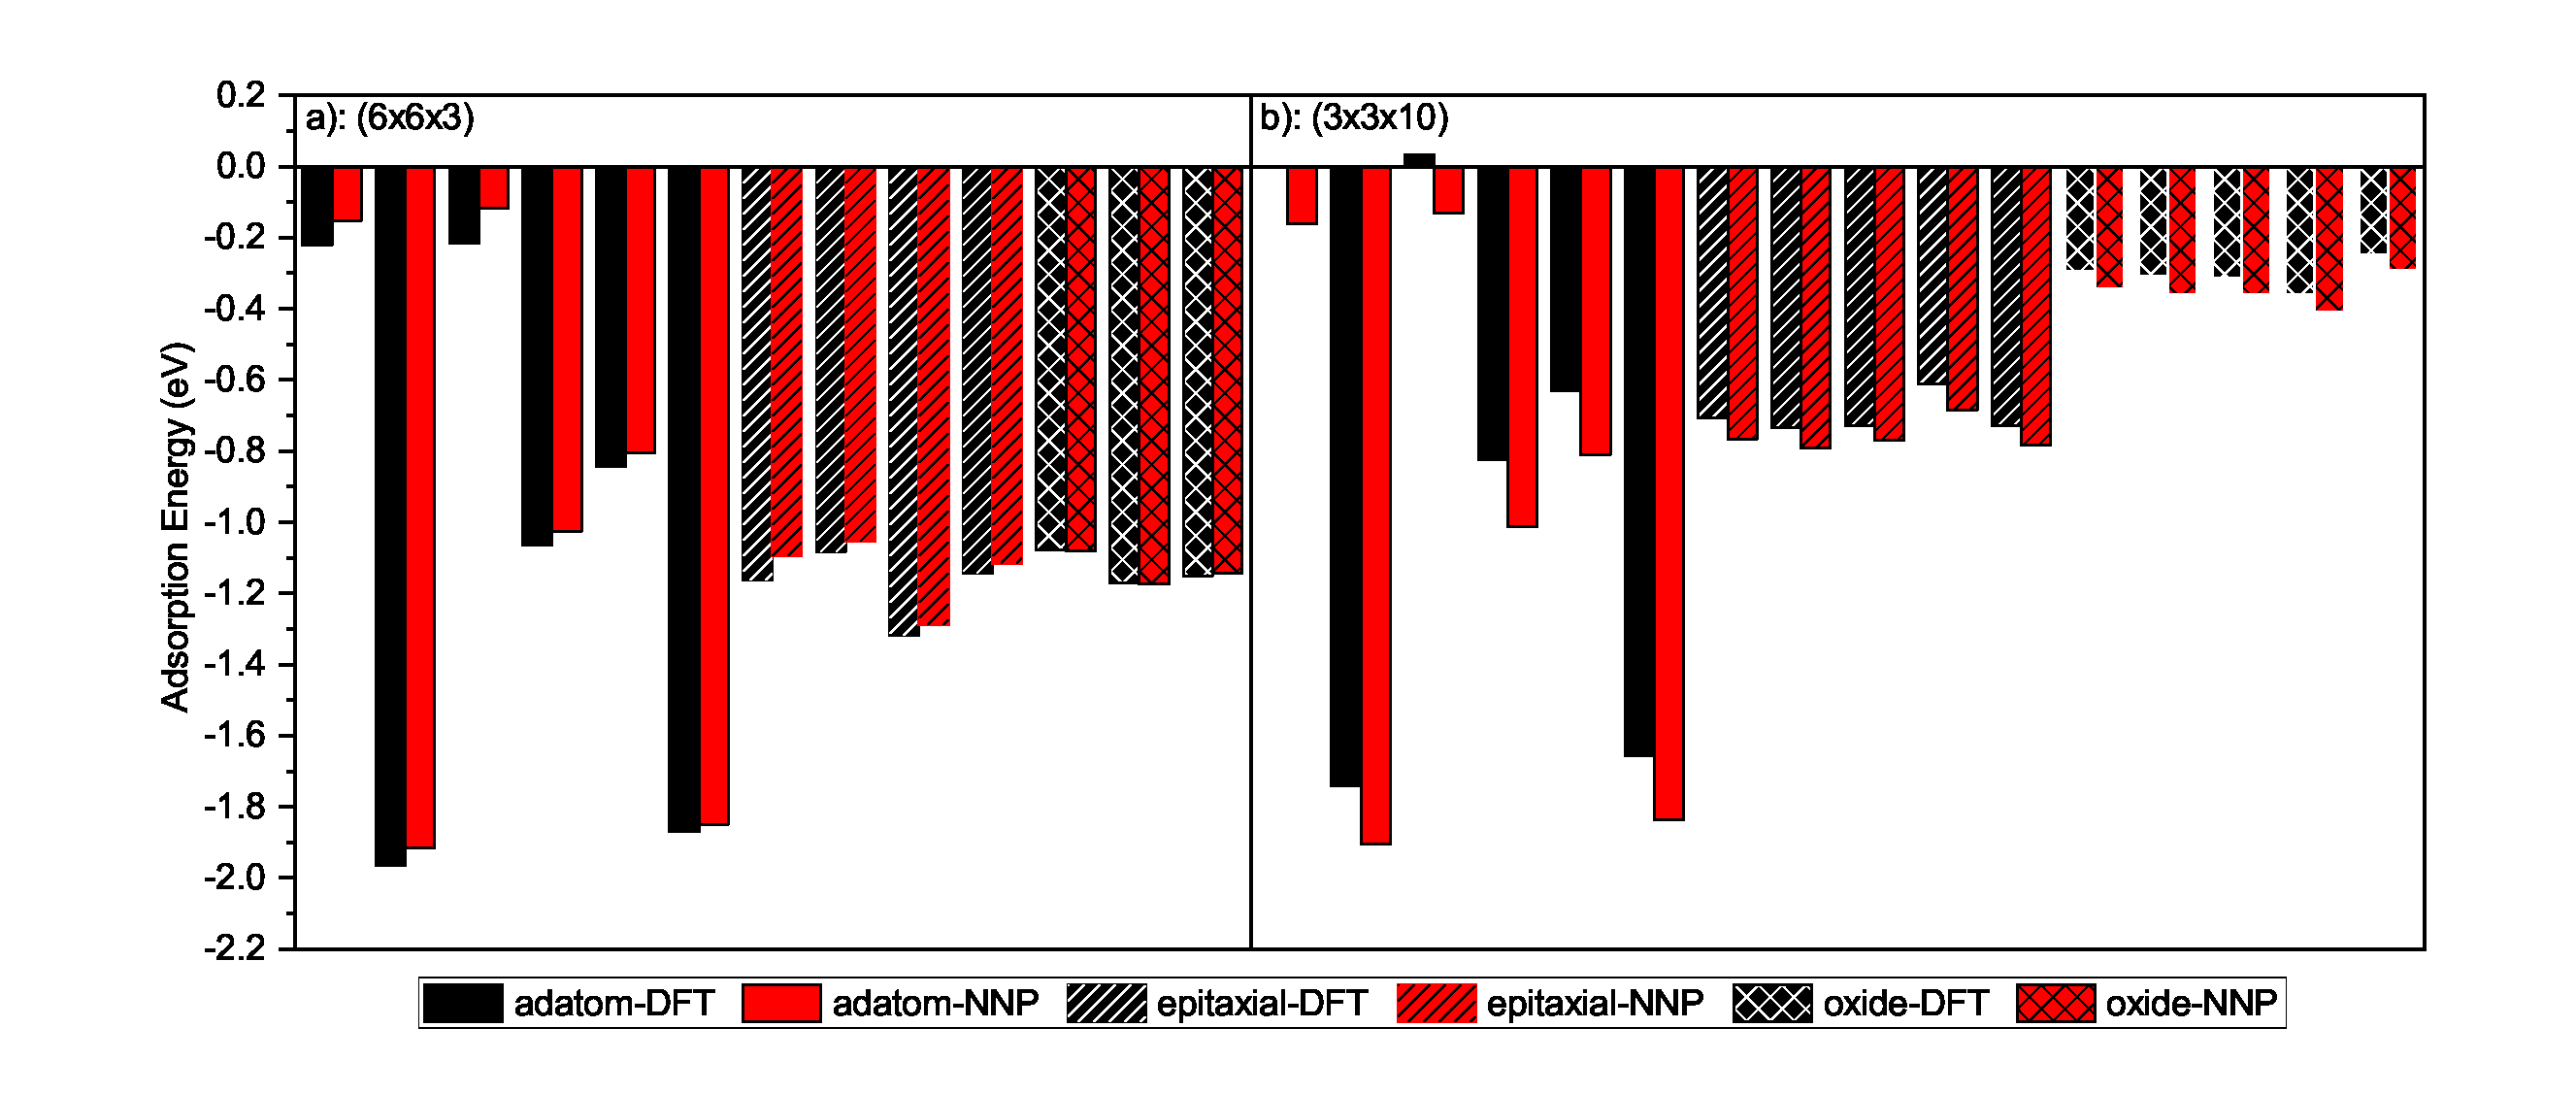
\includegraphics[width=\textwidth]{val_ads}
  \caption[Comparison of adsorption energies calculated using DFT and NNP]{}
  \label{fig:val_ads}
\end{figure}

The average adsorption energies on representative configurations from 3 different phases of oxidation are shown in Figure \ref{fig:ads}. Two types of slab structures are used: the $(6\times6\times3)$ slab and the $(3\times3\times10)$ slab. These structures are chosen as surrogates for the very large production size slabs, since the latter would be prohibitively expensive to calculate directly. Despite the adsorption being a stricter test than the error per atom, the final neural network performed remarkably well to give adsorption energies within \SI{0.1}{eV} for most of the configurations. In the worst case, the adsorption energy is within \SI{0.2}{eV} of the DFT value. This accuracy is close to the inherent error in DFT itself. As further validation, the transition states of oxygen and copper atom diffusion on Cu surfaces were calculated and compared with DFT values in the Figure \ref{fig:TS}. During the search for TS, the images of the reactant, the product, and the intermediate nudged elabstic band (NEB) images were independently optimized by the two methods to prevent structural correlation. It can be seen that the diffusion barrier calculated via the NNP lie within \SI{0.1}{eV} of the DFT predicted value. Thus, we conclude that our NNP can be used to simulate the ion impact trajectories at close-to-DFT accuracy.
\begin{figure}[h]
  \centering
  \includegraphics[width=\textwidth]{val_close}
  \caption[Comparison of the PES calculated using DFT and NNP on simulated impact event]{}
  \label{fig:val_close}
\end{figure}

% we are still missing plasma-specific validation data.

\bibliography{ref}    % bibliography references
\end{document}

%%% Local Variables:
%%% mode: latex
%%% Tex-engine: xetex
%%% TeX-master: t
%%% End:

\message{ !name(paper.tex) !offset(-164) }
